\section{Aggregating Induced Views}
\label{sec:aggregation}
In the previous sections, we introduced four strategies to identify the accepted answer to a question. Each strategy induces a graph or relational view between $(q,a)$ tuples.
%three relation types to connect $(q,a)$ tuples --- Contrastive, Similar Contrast and Reflexive. Each relation type has one or more induced views capturing relationships between $(q,a)$ tuples under a strategy. %We distinguish the relational class and a specific view such as TrueSkill, which is an instance of the Similarity class.
Each relational view is expected to capture semantically diverse neighborhoods of vertices. The convolution operator aggregates the neighborhood information under each view. The key question that follows is, \emph{how do we combine these diverse views in a unified learning framework?} Past work has considered multiple solutions:
\begin{itemize}
  \label{item:aggregator}
\item \textbf{Neighborhood Aggregation}: In this approach, we represent vertices by aggregating feature representations of it's neighbors across all views \cite{graphsage,relationalGCN}.
\item \textbf{Stacking}: Multiple convolution layers stacked end-to-end (each potentially handling a different view) \cite{Stacking}.
\item \textbf{Fusion}: Follows a multi-modal fusion approach~\cite{Fusion18}, where views are considered distinct data modalities.
\item \textbf{Shared Latent Structure}: Attempts to transfer knowledge across relational views (modalities) with constraints on the representations (e.g. \cite{DualGCN} aligns embeddings across views).
\end{itemize}

Ensemble methods introduced in \cite{relationalGCN} work on multi-relational edges in knowledge graphs. None of these approaches are directly suitable for our induced relationships. Our relational views utilize different label assignment semantics (label sharing within a clique vs. determine label based on contrast within a clique). In our label contrast semantics, we must achieve feature discrimination and label inversion between contrasting vertices, as opposed to label homogeneity and feature sharing in the label sharing case. Thus, aggregating relationships by pooling, concatenation, or addition of vertex representations fail to capture semantic heterogeneity of the induced views.
Further, data induced relations are uncurated and inherently noisy. Directly aggregating the learned representations via Stacking or Fusion can lead to noise propagation. We also expect views of the same relation type to be correlated.

%In our Contrastive strategy, we must achieve feature discrimination and label inversion between contrasting nodes, as opposed to label homogeneity and feature sharing in the Relative Similarity strategy. Gradient boosting techniques are known to improve performance when individual classifiers, including neural networks \cite{ncboost}, are diverse yet accurate. A natural solution then is to apply boosting to the set of IR-GCNs and bridge the weaknesses of each learner. However, a direct application across all views is sub-optimal as it does not exploit the commonalities within a strategy (e.g., The TrueSkill and Arrival Similarity views within Relative Similarity).

%\begin{itemize}
%\item \textbf{Consistency Viewpoint:} In this view, each relation GCN is though to produce precisely the same result in the ideal case, i.e., where they are all trained exhaustively on the chosen set of relations. Thus, the reduced performance is though to indicate incompleteness rather than inability. Namely, aligning the relation GCNs in a co-operative manner is thought to produce the best results. Recent work \cite{www2018} used local and global neighborhoods of nodes (by random-walk similarity) to construct a pair of aligned GCNs. They further introduced a regularization or result-alignment term in the loss function to improve their performance by leveraging each other's predictions.
%
%\item \textbf{Diversity Viewpoint:} Conversely, in this view, each relation GCN is though to fit to a different subset of the data points. For instance Contrast relation is likely to perform well in the presence of a single quality answer while True Skill similarity identifies the relative position of users in comparison to their peers. Unlike the pretvious case, the ideal outcome in the Diversity viewpoint is to learn completely disjoint relation GCNs, each of which perform well on some subset of the data or the input feature space. It is easy to bserve that the best strategy in this case is not to try and align the GCNs. Rather, we must effectively exploit their dissimilarities to obtain the best combined performance.
%\end{itemize}

\begin{figure}
    \centering
        %\includegraphics[width=\columnwidth,height=3cm]{figures/model.pdf}
    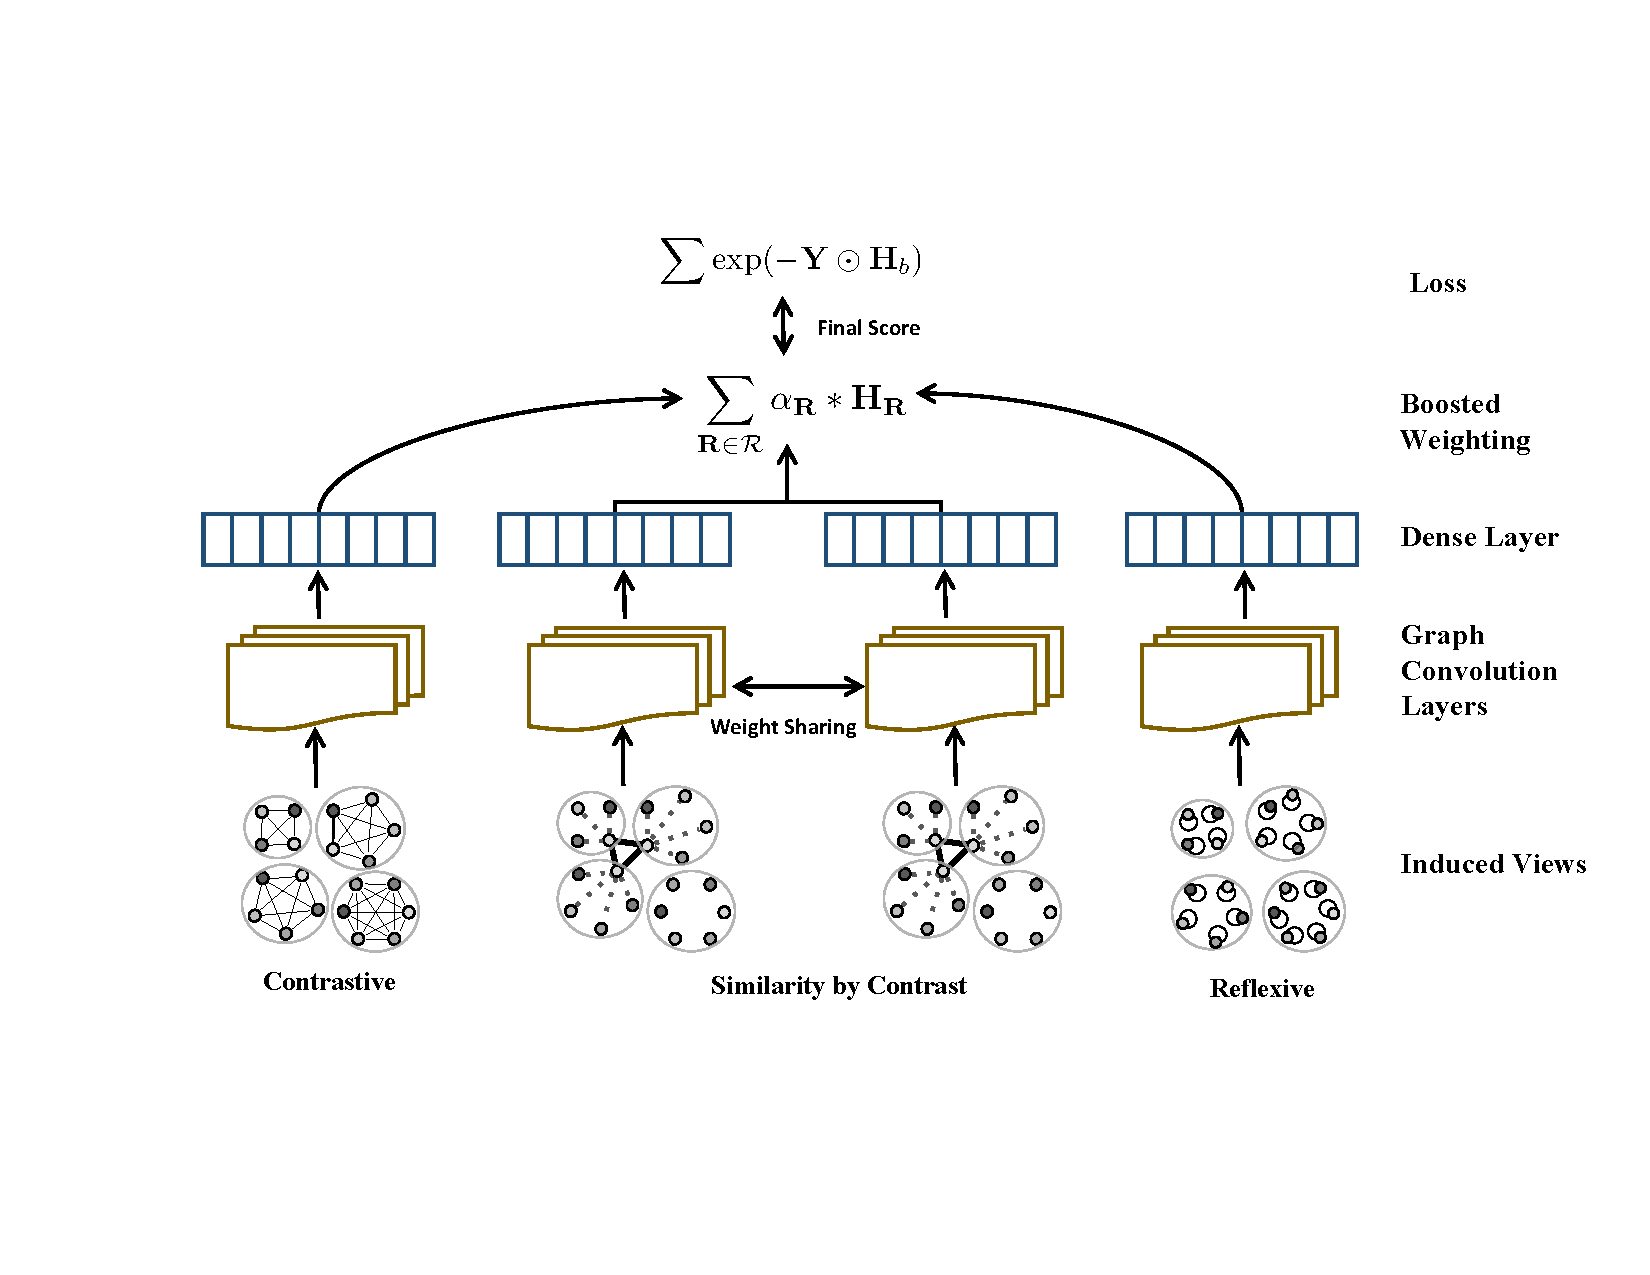
\includegraphics[scale=0.48]{figures/Architecture_new.pdf}
    %\includegraphics[scale=0.33]{figures/Architecture_dark.pdf}
    \caption{\small \label{fig:adaboost} Schematic diagram of our proposed IR-GCN model.} %The model is generic and can be extended to relational classes and multiple relational views within each class.}
    \vspace{-0.1in}
\end{figure}

%Consider the most general ontology of the chosen relations, namely a set of strategies (such as Contrastive and Similarity), each with multiple views (e.g. True Skill, Arrival).

We thus propose the following approach to aggregate information across relation types and between views of a relation type.

\noindent
\textbf{Cross-relation Aggregation}: We expect distinct relation types to perform well on different subsets of the set of $(q,a)$ tuples. We empirically verify this with the Jaccard overlap between the set of misclassified vertices under each relational view of a relation type on our dataset. Given $\mathbf{M}_A$ and $\mathbf{M}_B$, the sets of $(q,a)$ tuples misclassified by GCNs $A$ and $B$ respectively, the jaccard overlap is,
\begin{equation*}
 \mathcal{J}_{A,B} = \frac{\mathbf{M}_A \cap \mathbf{M}_B}{\mathbf{M}_A \cup \mathbf{M}_B}
\end{equation*}
The $\mathcal{J}_{A,B}$ values are as follows for the relational pairings: (Contrastive, TrueSkill Similarity) = 0.42, (Contrastive, Reflexive) = 0.44 and (Reflexive, TrueSkill Similarity) = 0.48. Relatively low values of the overlap metric indicate uncorrelated errors across the relations.

Gradient boosting techniques are known to improve performance when individual classifiers, including neural networks \cite{ncboost}, are diverse yet accurate. A natural solution then is to apply boosting to the set of relation types and bridge the weaknesses of each learner. We employ Adaboost \cite{adaboost} to combine relation level scores, $\mathbf{H}_{\mathbf{R}}$ (~\cref{eq:score}) in a weighted manner to compute the final boosted score, $\mathbf{H}_b \in \mathbb{R}^{N \times 1}$ representing all relation types (Line 12, ~\cref{alg:inference}). $\mathbf{Y} \in \mathbb{R}^{N X 1}$ denotes the acceptance label of all tuples. Note that an entry in $(\mathbf{Y} \odot \mathbf{H_{\mathbf{R}}}) > 0 $ when the accepted label of the corresponding $(q,a)$ tuple and sign of the prediction score, $sign(\mathbf{H_{\mathbf{R}}})$, of relation type $\mathbf{R}$ match and $< 0$ otherwise. Thus, the weights $\alpha_\mathbf{R}$ adapt to the fraction of correctly classified tuples to the misclassified tuples by the relation $\mathbf{R}$ (Line 9, ~\cref{alg:inference}).
%weight of each subsequent strategy's score is determined by the misclassification error, ($\mathbf{e}_\mathbf{S}$), of $(q, a)$ tuples by the current set of strategies.
The precise score computation is described in ~\cref{alg:inference}. We use the polarity of each entry in the boosted score, $sign(\mathbf{H}_b) \in \{-1,1 \}$, to predict the class label of the corresponding $(q,a)$ tuple. The final score is also used to create a ranked list among all the candidate answers, $a \in \mathcal{A}(q)$ for each question, $q \in \mathcal{Q}$. $L_{(q,a)}$ represents the position of candidate answer $a$ in the ranked list for question $q$.

%These class level outputs are then scaled and combined by the respective gradient boosting methods (we employed Adaboost \cite{adaboost} in our experiments)
\begin{algorithm}
\caption{IR-GCN Boosted Score Computation}\label{alg:inference}
\begin{algorithmic}[1]
%\Require{Nodes $x_1 \ldots x_n$, Class labels $y_1 \ldots y_n$, $y_i \in \{-1,1\}$, Adjacency matrix of each induced GCN $A_c, A_{ts}, A_{as}, A_r$}
%\Ensure{boosted score $h_b(x_i) \forall i \in [1, n]$}
\Function{Forward}{$\mathbf{X}, \mathbf{Y}, \{A_i\}_{S_i \in \mathbf{S}}$}
  \State $\mathbf{H}_{b} \gets \mathbf{0} $
    \For{$\mathbf{R} \in \mathcal{R}$}
    \State $\{ \mathbf{Z}_i^K \}_{S_i \in \mathbf{R}} \gets Conv(\mathbf{X}, \{ A_i \}_{S_i \in \mathbf{R}})$
    \State \Comment{Equation  \ref{eq:contrast}, \ref{eq:similar}, \ref{eq:reflexive}}
    \State $\mathbf{H}_\mathbf{R} =\sum_{{S_i} \in \mathbf{R}} \mathbf{Z}_i^{K} \times \widetilde{\mathbf{W}}_i$ \Comment{Equation \ref{eq:score}}
    %\State $h_s = merge(h_{as}, h_{ts})$ \Comment{Equation \ref{eq:merge}}
    \State $ \mathbf{e}_{\mathbf{R}} \gets \exp({-\mathbf{Y} \odot \mathbf{H}_{b}})$
    \State \Comment{ $\odot \rightarrow \textit{Hadamard Product}$}
  \State $\alpha_\mathbf{R} \gets \dfrac{1}{2} \ln{\dfrac{\sum \mathbf{e}_{\mathbf{R}} \odot \mathbbm{1}\left((\mathbf{Y} \odot \mathbf{H}_{\mathbf{R}}\right) > 0)}{\sum \mathbf{e}_{\mathbf{R}} \odot \mathbbm{1}\left((\mathbf{Y} \odot \mathbf{H}_{\mathbf{R}}) < 0 \right) }}$
    \State \Comment{$\sum \rightarrow \textit{reduce-sum}$}
      \State \Comment{$\mathbbm{1}(.) \rightarrow \textit{element-wise Indicator function}$}
  \State    $\mathbf{H}_{b} \gets \mathbf{H}_{b} + \alpha_\mathbf{R} * \mathbf{H}_{\mathbf{R}}$ \Comment{Update boosted GCN}
%    \State $ w_{i,r} \gets \exp^{-y_i * h_{cs}(x_i)}$
%  \State    $\alpha_r \gets \dfrac{1}{2} \lnb{\dfrac{\sum\limits_{y_i = h_s(x_i)} w^{i,c}}{\sum\limits_{y_i \neq h_s(x_i)} w_{i,c} }}$
%    \State $h_{b}(x_i) \gets h_{cs}(x_i) + \alpha_r * h_{cs}(x_i)$\Comment{Final Boosted GCN}
    \EndFor
    \State \Return $\mathbf{H}_{b}$, $ \{ \mathbf{H}_{R} \}_{\mathbf{R} \in \mathcal{R}}$, $\{ \mathbf{Z}_{i}^{K} \}_{S_i \in \mathbf{S}}$
    \State \Comment{Boosted scores, Relation level scores,}
    \State \Comment{Each GCN vertex representations}
\EndFunction
\end{algorithmic}
\end{algorithm}

%Now we describe the boosted weights for the outputs of each relational view for each tuple $t_{i}$, namely $h_{\mathcal{C}}(t_{i})$. The weights $w_{\mathcal{C}}(t_i)$ of the $t_i^{th}$ tuple for the $\mathcal{C}^{th}$ relational view are given by $w_{\mathcal{C}}(t_i) = e^{-y_{i}\times h_{(1 \ldots \mathcal{C}-1)}(t_i)}$, where $h_{(1 \ldots \mathcal{C}-1)}$ denotes the prediction output of the boosted classifier combining all relational views before view $\mathcal{C}$. In our answer selection problem, the contrastive relational view performs the best, and is hence added first to the ensemble, followed by relative similarity and reflexive views, i.e. $\{c,s,r\}$. The above description is formalized in \cref{alg:inference}.

\noindent
\textbf{Intra-relation Aggregation}: Gradient boosting methods can effectively aggregate relation level representations, but are not optimal within a relationship type (since it cannot capture shared commonalities between different views of a relation type). For instance, we should facilitate information sharing between the TrueSkill similarity and Arrival similarity views. Thus, if an answer is authored by a user with a higher skill rating and answered significantly earlier than other answers, its probability to be accepted should be mutually enhanced by both signals. Empirically, we also found True Skill and Arrival Similarity GCNs to commit similar mistakes ($\mathcal{J}_{TS,AS}$ = 0.66). Thus, intra-relation learning (within a single relation type like Similarity by Contrast) can benefit from sharing the structure of their latent spaces, i.e., weight parameters of GCN.

%We also share the weight matrices $W_{v}^{k} \forall k \in [1,\ldots,K]$ to enable analogous data transformations between TrueSkill and Arrival Similarity.



%Motivated by the regularization term in \cite{DualGCN}, we follow a similar strategy to combine our similiarity view IR-GCNs. Now consider a relational view $\mathcal{C}$ with instances $v \in \mathcal{C}$ (e.g. TrueSkill, Arrival in the Similarity view). To share the latent structure of their representations, the following regularizer is introduced ($t_i$ denotes a single $(q,a)$ tuple),
%\begin{equation}
%\sum_{i}\sum_{(v, v') \in \mathcal{C}} || Z_v^{K}(t_i) - Z_{v'}^{K}(t_i) ||
%\end{equation}
%The embedding representations are constrained to be similar at the last layer (k=K) for all pairs of instances in a view.


%We provide the details of our training algorithms in \cref{sec:aggregation}.

%In the previous sections we described three relational views, Contrastive (c), Similarity (s) and Reflexive (r). For each view $\mathcal{C} \in \{c,s,r\}$, we have a set of instances $v \in \mathcal{C}$ and each IR-GCN$_{v}$ generates embedding representation $Z_{v}^{K}(t_i)$.
%These class level outputs are then scaled and combined by the respective gradient boosting methods (we employed Adaboost \cite{adaboost} in our experiments). Figure \ref{fig:adaboost} exhibits the overall architecture of our Boosted IR-GCN model. The above description is formalized in \cref{alg:inference}.
\noindent
\emph{Weight Sharing:} For multiple views representing a relation type (e.g., TrueSkill and Arrival Similarity), we train a separate GCN for each view but share the layer-wise linear-transforms $\mathbf{W}_i^{k}$ to capture similarities in the learned latent spaces.
Weight sharing is motivated by a similar idea explored to capture local and global views in \cite{DualGCN}. Although sharing the same weight parameters, each GCN can still learn distinct vertex representations as each view convolves over a different neighborhood and employ random dropout during training.
%Thus, in practice, each view can potentially predict opposite class labels.
We thus propose to use an alignment loss term to minimize prediction difference between views of a single relation type\cite{reg}. The loss attempts to align the learned vertex representations at the \emph{last layer} $K$ (the loss term aligns pairs of final vertex representations, $\lvert\lvert \mathbf{Z}_i^{K} - \mathbf{Z}_{i'}^{K} \lvert\lvert \texttt{  }\forall\texttt{ } S_i, S_i' \in \mathbf{R}$). In principle, multiple GCNs augment performance of the relation type by sharing prior knowledge through multiple Adjacency matrices ($\mathbf{A}_i \texttt{  }\forall\texttt{ } S_i \in \mathbf{R}$).
%weight sharing and alignment loss.


\begin{algorithm}[tbh]
\caption{IR-GCN Training}\label{alg:training}
\begin{algorithmic}[1]
\Require{Input Feature Matrix $X$, Acceptance labels for each tuple, $\mathbf{Y}$, Adjacency matrix of each view $\{A_i\}_{S_i \in \mathbf{S}}$ }
\Ensure{Trained Model i.e. Weight parameters $W_{i}^{1} \ldots W_{i}^{k}, S_i \in \mathbf{S}, \forall k \in [1, K]$ and transform parameters $\widetilde{W}_i$, $S_i \in \mathbf{S}$ }
%\Ensure{Trained Model i.e. Weight parameters $W_{\mathbf{S}}^{1} \ldots W_{\mathbf{S}}^{k}, \mathbf{S} \in %\mathbb{S} $ and transform parameters $\widetilde{W}_v$, $v \in \mathbf{V}$ }
%\While{ $not$ $converged$}
%\For{$t\gets0 to \textit{num_epochs}$ }
\For{$t \gets 1$ to $\textit{num-epochs}$}
    \State $\mathbf{H}_b, \{ \mathbf{H}_{R} \}_{\mathbf{R} \in \mathcal{R}}, \{ \mathbf{Z}^{K}_{i} \}_{S_i \in \mathbf{S}}$$\gets \textsc{Forward}(X, Y, \{ A_i \}_{S_i \in \mathbf{S}})$
    \State \Comment{\Cref{alg:inference}}
    \For{ $\mathbf{R} \in \mathcal{R}$}

        \State $\mathcal L_b \gets \sum \exp({-\mathbf{Y} \odot \mathbf{H}_b}) + \gamma_1 \mathcal L_1(.) + \gamma_2 \mathcal L_2(.)$
    \State \Comment{$\sum \rightarrow \textit{reduce-sum}$}
  \State \Comment{$\odot \rightarrow \textit{Hadamard Product}$}
        \State $\mathcal L_{\mathbf{R}} \gets 0$
        \For{ $S_i \in \mathbf{R}$}
        \State $\mathcal L_{i} \gets \sum \exp({-\mathbf{Y} \odot \mathbf{H}_\mathbf{R}})$
                    %\State \Comment{$\sum \rightarrow \textit{reduce-sum}$}
    \State $\mathcal L_{\mathbf{R}} \gets \mathcal L_{\mathbf{R}} + \mathcal L_{i} + \frac{1}{2}\sum_{S_i' \neq S_i}\lvert\lvert \mathbf{Z}_{i}^K - \mathbf{Z}_{i'}^K \lvert\lvert $
    \EndFor
    \State $\mathcal L_b \gets \mathcal L_b + \lambda(t) \mathcal L_{\mathbf{R}}$
    \State    $W_i^{k} \gets  W_i^{k} + \eta_{\textsc{adam}} \frac{\partial \mathcal L_b}{\partial W_i^{k}} $ \Comment{$\forall k \in [1, K], \forall S_i \in \mathbf{R}$}
     \State    $\widetilde{W}_i \gets  \widetilde{W}_i +  \eta_{\textsc{adam}} \frac{\partial \mathcal L_b}{\partial \widetilde{W}_i}$ \Comment{$\forall S_i \in \mathbf{S}$}
    \EndFor
\EndFor
\end{algorithmic}
\end{algorithm}

%\subsection{Training algorithm}
\noindent
\textbf{Training Algorithm}: Algorithm \ref{alg:training} describes the training algorithm for our IR-GCN model. For each epoch, we first compute the aggregated prediction score $\mathbf{H}_{b}$ of our boosted model, as described in \cref{alg:inference}. We use a supervised exponential loss $\mathcal{L}_b$ for training with elastic-net regularization (L1 loss - $\mathcal L_1(.)$ and L2 loss - $\mathcal L_2(.) $) on the graph convolutional weight matrices $\mathbf{W}_{\mathbf{i}}^{k} \texttt{  }\forall\texttt{ } S_i \in \mathbf{S}$ for each view. Note that we employ weight sharing between all views of the same relation type so that only one set of weight matrices is learned per relation. %The views in our training are Contrast (c), TrueSkill (ts), Arrival Similarity (as), and Reflexive view (r).
The exponential loss, $\mathcal{L}_{\mathbf{R}}$, for each relation type is added alternatingly to the boosted loss.
We apply an \emph{exponential annealing schedule}, $\lambda(t)$, i.e. a function of the training epochs ($t$), to the loss function of each relation. As training progress and the boosted model learns to distribute vertices among the relations optimally, an increase in $\lambda(t)$ ensures more emphasis is provided to the individual convolutional networks of each relation. Figure \ref{fig:adaboost} illustrates the overall architecture of our IR-GCN model.

%\textbf{IR-GCN Annealing}:
%Note that the regularizer $\lvert\lvert Z_{as} - Z_{ts} \lvert\lvert$ ensures close coupling between the embeddings learned between views of the same strategy. F %The final output score of similarity relation is then computed by aggregating information from both relations as in Equation \ref{eq:merge}.




%We now consider Intra-class aggregation.

% Now we describe the boosted weights for the outputs of each relational view for each tuple $t_{i}$, namely $h_{\mathcal{C}}(t_{i})$. The weights $w_{\mathcal{C}}(t_i)$ of the $t_i^{th}$ tuple for the $\mathcal{C}^{th}$ relational view are given by $w_{\mathcal{C}}(t_i) = e^{-y_{i}\times h_{(1 \ldots \mathcal{C}-1)}(t_i)}$, where $h_{(1 \ldots \mathcal{C}-1)}$ denotes the prediction output of the boosted classifier combining all relational views before view $\mathcal{C}$. In our answer selection problem, the contrastive relational view performs the best, and is hence added first to the ensemble, followed by relative similarity and reflexive views, i.e. $\{c,s,r\}$. The above description is formalized in \cref{alg:inference}.


%Gradient boosting techniques are known to improve performance when individual classifiers, including neural networks \cite{ncboost}, are diverse yet accurate. This precisely fits our inter-class aggregation problem. The aggregate of the strongest relational class is added first to the ensemble, and adaptive weights are applied for each subsequent relational class to leverage the misclassified nodes of the current boosted classifier, hence satisfying the diversity viewpoint.



% Each $v^{th}$ IR-GCN produces an output score $h_v(t_i) \in [ -1, 1 ]$ for each tuple $t_i$. We obtain this score by projecting learned node embeddings $Z_m(x_i)$ for each IRGCN to a single value.
%\begin{equation}
%    \label{eq:score}
%        h_m(x_i) = Z_m(x_i) * \tilde{W}_m; \forall m \in \{ c, ts, as, r\}
%\end{equation}
%with $\tilde{W}_m \in \mathbb{R}^{K X 1}$ and output embedding size $K$. If there are multiple induced relations for a relationship type, final score is computed by concatenating scores of each induced-relation GCN model. For instance, for similarity relation, final score $h_s(x_i)$ is computed as,
%\begin{equation}
%    \label{eq:merge}
%    h_s(x_i) = [h_{ts}(x_i), h_{as}(x_i)]* \tilde{W}_{concat}
%\end{equation}
%where $h_{ts}$ is true skill similarity GCN score, $h_{as}$ is arrival similarity GCN score with $\tilde{W}_{concat} \in \mathbb{R}^{2 X 1}$.


%\vspace{-0.2in}
%We then combine these individual $h_m$ scores to compute final score of our boosted Induced-Relation GCN model as defined in Algorithm \ref{alg:inference}. We define weight $w_m^{(i)}$ of $m$th weak learner for node $x_i$ as the exponential loss over $m-1$th weak learner's score:
%\begin{equation}
%    \label{eq:weight}
%        w^{(i)}_m = \exp^{-y_i * h_{m-1} (x_i)}
%    \end{equation}
%For our answer selction problem, contrastive GCN is the strongest individual learner followed by similarity and reflexive GCN. We then compute weight for second weak learner, similarity GCN $w_s^{(i)}$ using line 7 in Algorithm \ref{alg:inference}. The weight of node $x_i$ for similarity GCN increases as the score of contrastive GCN $h_c$ is further away from the true label $y_i$. Final combined weight for similarity GCN learner $\alpha_s$ is proportional to the ratio of sum of weights $w_{i,s}$ for nodes $x_i$ correctly classified by similarity GCN with the sum of weights of misclassified nodes. This combined weight, hence, ensures that similarity GCN trains better for nodes misclassified by the contrastive GCN. The intermediate boosted score $h_{cs}$ is then defined as a weighted sum of Contrastive GCN score $h_c$ and Similarity GCN score $h_s$ in Line 9. The same process is repeated for reflexive learner where weight is determined using misclassification errors of the intermediate boosted learner. Line 12 specifies the final score for boosted induced-relation GCN $h_b$.

%
% \begin{algorithm}[H]
% \caption{Sum of Array Elements}
% \label{alg:loop}
% \begin{algorithmic}[1]
% \Require{Nodes $x_1 \ldots x_n$, Class labels $c_1 \ldots c_n$ ,$c_i \in \{-1,1\}$, Output of each induced GCN $h_c, h_s, h_r$ $\forall h: x \rightarrow \{ -1, 1 \}$}
% \Ensure{$h_G$ (Final label for each node)}
% \Statex
% \Function{Loop}{$A[\;]$}
%   \State {$Sum$ $\gets$ {$0$}}
%     \State {$N$ $\gets$ {$length(A)$}}
%     \For{$k \gets 1$ to $N$}
%         \State {$Sum$ $\gets$ {$Sum + A_{k}$}}
%     \EndFor
%     \State \Return {$Sum$}
% \EndFunction
% \end{algorithmic}
% \end{algorithm}
%\setlength{\textfloatsep}{1pt}
%The contrastive, similarity and reflexive relations capture different facets of question-answer pairs as a function of their competitors, similar tournaments and self-features. Each induced relationship captures a different data characteristic and the convolution operation aggregates neighborhood information from each of these relationships. The key question that follows is, how do we combine these diverse sources of relationship information in a unified learning framework? We first analyze the relative strengths of each learner by comparing the set of nodes they can correctly classify when applied in isolation.
% A combined classification model could thus outperform individual learners by a wide margin.
%
%%Thus, it is important to combine these different information to build an effective classification model.
%%To verify correlation between these relationships, we compute Jaccard Coefficient between the misclassified nodes of Contrastive, True Skill Similarity and Reflexive GCN model.
%Total loss of our proposed model is then defined as weighted sum of boosted model loss $\mathcal L_b$ with loss for similarity relation GCN. The weight for similarity GCN $\lambda(t)$ increases exponentially with $t$ epochs. This ensures that at the beginning of training, boosted induced-relation GCN is trained as it dominates the loss function. While as training progresses and boosted IRGCN model learns distribution of nodes among each IRGCN, increase in $\lambda(t)$ ensures similarity GCN to be trained for those assigned nodes to mutually enhanced by each other.
%
%//, by using multiple neural networks, different prior
%knowledge can be embedded during the data transformation stage.
